\chapter{La geometría del espacio homogéneo}

\lectureoverview{La planitud es una excelente aproximación al universo observado, pero no es un principio. Si mantenemos la homogeneidad y la isotropía y permitimos la curvatura, aparecen tres geometrías espaciales simplemente conexas: el espacio euclídeo, el esférico y el hiperbólico. Sus métricas pueden construirse a partir del crecimiento de capas concéntricas con la distancia, y su curvatura puede ponerse a prueba mediante los tamaños angulares y el recuento de objetos. El espacio plano también puede ser finito si su topología es toroidal. Por último, al asociar un factor de escala dependiente del tiempo a cualquiera de estos espacios homogéneos se obtienen las métricas cosmológicas del espacio-tiempo y la ley de Hubble; la dinámica de ese factor de escala debe derivarse de la relatividad general.}

\section{La planitud es una observación, no un principio}

Hasta ahora hemos tratado el espacio como plano y apenas hemos hablado de la geometría del espacio-tiempo. Las observaciones justifican considerar el espacio plano como una muy buena aproximación, pero no convierten la planitud en una ley. Lo que realmente nos dicen las mediciones es que cualquier radio de curvatura debe ser grande en comparación con la región que hemos cartografiado. El espacio podría ser exactamente plano, tener curvatura positiva o tener curvatura negativa. A escalas muy superiores a la región observable, todavía no sabemos cuál de estas descripciones es correcta.

Por tanto, relajaremos un supuesto y mantendremos otro. No supondremos que el espacio es plano, pero seguiremos suponiendo que es homogéneo e isotrópico. Se trata de una hipótesis de trabajo, no de un artículo de fe. Para averiguar sus consecuencias, la suponemos y calculamos; después podremos abandonarla y preguntarnos qué diferencias habría en un universo inhomogéneo.

La homogeneidad significa que todos los puntos tienen el mismo carácter geométrico. Un observador que se desplace a otro lugar y repita experimentos geométricos locales obtendrá los mismos resultados. La isotropía significa que no hay ninguna dirección preferida. Estas condiciones excluyen casi todas las superficies curvas que dibujamos primero. Un paraboloide está más curvado cerca de su vértice que lejos de él. Un elipsoide alargado difiere en los polos y en el ecuador. Una esfera irregular, o la superficie terrestre si se resuelven sus montañas y valles, es curva pero no homogénea. La pregunta cosmológica es más acotada:
\begin{quote}
¿Qué espacios pueden ser curvos y, aun así, tener el mismo aspecto geométrico desde todos los puntos y en todas las direcciones?
\end{quote}

Si por el momento ignoramos las identificaciones globales, hay tres respuestas de curvatura constante: el espacio plano, el espacio esférico de curvatura positiva y el espacio hiperbólico de curvatura negativa. La salvedad sobre las identificaciones globales es importante: más adelante construiremos un toro plano finito y corregiremos la afirmación demasiado simplificada de que estas tres opciones agotan todas las posibilidades.

\section{La métrica y las coordenadas del observador}

Primero hablaremos solo del espacio, no del espacio-tiempo. Su geometría está codificada en una métrica: una regla para calcular la distancia al cuadrado \(ds^2\) entre puntos vecinos. Una vez conocida esa regla local en todas partes, de ella pueden obtenerse las longitudes, los ángulos, las áreas, los volúmenes, las geodésicas y la curvatura.

En un plano euclídeo y en el espacio euclídeo tridimensional, las coordenadas cartesianas dan
\begin{equation}
ds_2^2=dx^2+dy^2,
\qquad
ds_3^2=dx^2+dy^2+dz^2.
\label{eq:c03-cartesian-flat}
\end{equation}
Añadir la tercera dimensión solo añade el término ortogonal \(dz^2\), pero lo importante no es la sencillez de esta fórmula. Lo importante es que la ecuación~\eqref{eq:c03-cartesian-flat} especifica por completo la geometría local.

\begin{figure}[htbp]
\centering
\includegraphics[width=0.74\textwidth]{lecture_03_figure_02.png}
\caption{La métrica cartesiana del espacio plano tridimensional, tal como está escrita en la pizarra.}
\label{fig:c03-cartesian-board}
\lectureframe{00:05:13.138}
\end{figure}

Las coordenadas cartesianas ocultan la manera en que un astrónomo encuentra el universo. Ocupamos un punto, miramos hacia fuera en distintas direcciones y clasificamos lo que vemos según el ángulo y la distancia. En un universo bidimensional, el campo visual sería literalmente un círculo de direcciones a nuestro alrededor. Por eso, las coordenadas polares no son solo elegantes: ponen de manifiesto la geometría angular que usa la cosmología.

Sea \(r\) la distancia radial y \(\theta\) la dirección. El mismo plano euclídeo tiene ahora la métrica
\begin{equation}
ds^2 = dr^2 + r^2 d\theta^2.
\label{eq:c03-polar-flat}
\end{equation}
Para un ángulo pequeño fijo \(d\theta\), la separación transversal es \(r\,d\theta\). Crece linealmente al alejarnos, por lo que su contribución al cuadrado de la métrica es \(r^2d\theta^2\).

El término angular es, por sí mismo, la métrica de un espacio unidimensional. Un círculo es una esfera unidimensional, denotada por \(S^1\), y la métrica del círculo unitario se escribe convencionalmente
\begin{equation}
d\Omega_1^2 = d\theta^2,
\qquad\text{so that}\qquad
ds^2 = dr^2 + r^2 d\Omega_1^2.
\label{eq:c03-omega-one}
\end{equation}
En la pizarra aparece \(d\Omega^2\) sin un subíndice legible; la definición oral precisa que el objeto previsto es \(d\Omega_1^2\).

\begin{figure}[htbp]
\centering
\includegraphics[width=0.74\textwidth]{lecture_03_figure_03.png}
\caption{Esquema y métrica de las coordenadas polares del espacio plano. En la pizarra aparece \(d\Omega^2\); la explicación lo identifica como la métrica del círculo unitario \(d\Omega_1^2=d\theta^2\).}
\label{fig:c03-polar-board}
\lectureframe{00:08:37.254}
\end{figure}

\begin{figure}[htbp]
\centering
\begin{tikzpicture}[scale=1.2]
\draw[->] (-1.2,0)--(1.8,0);
\draw[->] (0,-1.2)--(0,1.8);
\draw[thick] (0,0)--(1.3,1.1);
\draw (0.7,0.7) node[above] {$r$};
\draw (0.58,0) arc (0:40:0.58);
\draw (0.8,0.22) node {$\theta$};
\end{tikzpicture}
\caption{Reconstrucción limpia de las coordenadas polares centradas en el observador que se usan en la ecuación~\eqref{eq:c03-omega-one}.}
\label{fig:c03-polar-redraw}
\end{figure}

\begin{classroomqa}\audiencequestion{¿Mide realmente \(d\theta^2\) la distancia a lo largo de la circunferencia?}\lecturerresponse{Sí. En un círculo unitario, la longitud de arco es igual al ángulo medido en radianes, así que dos puntos vecinos separados por \(d\theta\) tienen una separación intrínseca al cuadrado de \(d\theta^2\). La circunferencia del círculo es \(2\pi\), y al integrar \(ds=d\theta\) una vuelta completa se obtiene precisamente \(2\pi\). Al multiplicar por \(r^2\), el círculo unitario se amplía hasta formar la capa de radio \(r\) en el plano. \lecturetimestamp{00:09:11--00:09:26}}\end{classroomqa}

La palabra \emph{intrínseca} es esencial. Si incrustamos el círculo unitario en un plano euclídeo, podemos describirlo mediante
\begin{equation}
x^2 + y^2 = 1.
\end{equation}
Esa ecuación describe cómo está situado el círculo en un espacio mayor. No la necesita quien vive en él y solo puede medir distancias a lo largo del círculo. Podríamos doblar una fibra óptica flexible hasta formar un lazo cerrado irregular sin estirarla. Su aspecto en el plano cambiaría, pero su circunferencia intrínseca y su métrica no. Incrementos iguales de \(\theta\) seguirían señalando distancias iguales a lo largo de la fibra. Por tanto, hay que separar la geometría de la forma accidental que le da una incrustación.

\begin{figure}[htbp]
\centering
\includegraphics[width=0.64\textwidth]{lecture_03_figure_04.png}
\caption{La pizarra compara un círculo unitario redondo con un lazo cerrado deformado. Si se dobla el lazo sin estirarlo, ambos tienen la misma métrica intrínseca unidimensional.}
\label{fig:c03-intrinsic-board}
\lectureframe{00:10:34.205}
\end{figure}

\begin{figure}[htbp]
\centering
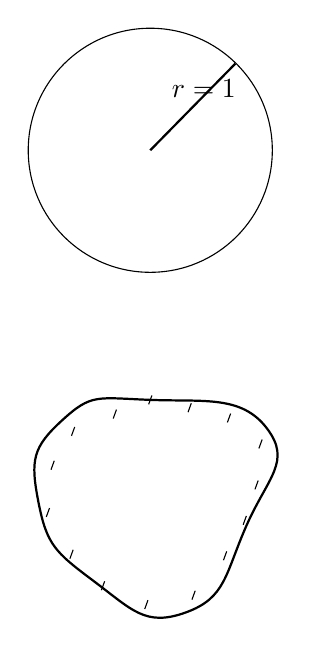
\begin{tikzpicture}[scale=1.0]
\draw (0,0) circle (1.55);
\draw[thick] (0,0)--(1.08,1.1);
\draw (0.68,0.78) node {$r=1$};

\begin{scope}[yshift=-4.35cm]
\draw[thick]
plot[smooth cycle, tension=0.95] coordinates
{(0,1.18) (1.48,0.82) (1.22,-0.42) (0.45,-1.52) (-0.72,-1.12) (-1.42,-0.12) (-1.12,0.92)};
\foreach \p in {(0,1.18),(0.5,1.08),(1.0,0.95),(1.4,0.62),(1.35,0.1),(1.2,-0.35),(0.95,-0.8),(0.55,-1.3),(-0.05,-1.42),(-0.6,-1.18),(-1.0,-0.78),(-1.3,-0.25),(-1.24,0.35),(-0.98,0.78),(-0.45,1.0)}{
\draw[rotate around={70:\p}] \p ++(-0.06,0) -- ++(0.12,0);
}
\end{scope}
\end{tikzpicture}
\caption{La distancia intrínseca se conserva al deformar la forma extrínseca: un observador unidimensional mide la misma circunferencia en ambas incrustaciones.}
\label{fig:c03-intrinsic-redraw}
\end{figure}

Ahora podemos interpretar el espacio plano como una familia anidada de círculos alrededor del observador. La capa a distancia \(r\) es una copia del círculo unitario ampliada por \(r\), que es precisamente lo que expresa el factor \(r^2d\Omega_1^2\).

\section{Curvatura positiva: capas que se cierran}

Una esfera es curva pero homogénea: ningún punto de una esfera perfectamente redonda se distingue geométricamente de los demás. Podemos construir su métrica sin recurrir a una representación externa en tres dimensiones. Imaginemos astrónomos bidimensionales que viven en una esfera unitaria \(2\) y sitúan el origen de sus coordenadas en su propia posición.

El círculo situado a una pequeña distancia geodésica \(r\) de ellos es pequeño. A medida que \(r\) aumenta, los círculos crecen, alcanzan su circunferencia máxima a mitad de camino alrededor de la esfera y luego se encogen hasta colapsar en el punto antipodal. Este crecimiento y contracción ocurren con la \emph{distancia}, no con el tiempo. La esfera permanece estática durante toda esta construcción.

Aquí \(r\) es la distancia angular a lo largo de la esfera unitaria, no la distancia euclídea desde un centro:
\[
0 \le r \le \pi.
\]
El origen elegido está en \(r=0\), el círculo máximo que la rodea a mitad de camino está en \(r=\pi/2\) y el punto antipodal, en \(r=\pi\). El radio de la capa es ahora \(\sin r\), así que el factor plano \(r^2\) se sustituye por \(\sin^2r\):
\begin{equation}
d\Omega_2^2 = dr^2 + \sin^2 r\, d\Omega_1^2
            = dr^2 + \sin^2 r\, d\theta^2.
\label{eq:c03-two-sphere}
\end{equation}
Los extremos y el punto medio se comportan exactamente como se requiere:
\begin{equation}
\sin 0=0,
\qquad
\sin\frac{\pi}{2}=1,
\qquad
\sin\pi=0.
\end{equation}
Así, las capas empiezan con tamaño cero, alcanzan su tamaño máximo y vuelven a cerrarse.

\begin{figure}[htbp]
\centering
\includegraphics[width=0.82\textwidth]{lecture_03_figure_05.png}
\caption{El paso de círculos anidados en el espacio plano a capas sobre la esfera. La fórmula inferior está parcialmente oculta en la imagen; su derivación oral da la sustitución \(r^2\mapsto\sin^2r\) en la ecuación~\eqref{eq:c03-two-sphere}.}
\label{fig:c03-spherical-board}
\lectureframe{00:16:11.701}
\end{figure}

\begin{figure}[htbp]
\centering
\resizebox{\linewidth}{!}{%
\begin{tikzpicture}[scale=0.92]
\begin{scope}[xshift=-4.15cm]
\draw[->] (-1.7,0)--(1.9,0);
\draw[->] (0,-1.7)--(0,1.9);
\draw (0,0) circle (0.45);
\draw (0,0) circle (0.9);
\draw (0,0) circle (1.35);
\draw[thick] (0,0)--(1.45,1.2);
\draw (0.56,0.18) arc (18:40:0.63);
\draw (0.94,0.44) node {$\theta$};
\end{scope}

\begin{scope}[xshift=4.15cm]
\draw (0,0) circle (2.0);
\fill (0,-2.0) circle (1.5pt);
\fill (2.0,0) circle (1.5pt);
\fill (0,2.0) circle (1.5pt);
\draw[thick] (0,-2.0) arc (-90:90:2.0);
\draw (0,-2.35) node {$r=0$};
\draw (2.75,0) node {$r=\pi/2$};
\draw (0,2.35) node {$r=\pi$};
\end{scope}
\end{tikzpicture}
}%
\caption{Las capas planas crecen indefinidamente, mientras que las esféricas alcanzan su tamaño máximo en \(r=\pi/2\) y se cierran en \(r=\pi\).}
\label{fig:c03-shells-flat-sphere}
\end{figure}

La notación \(d\Omega_2^2\) significa la métrica de la esfera unitaria \(2\), del mismo modo que \(d\Omega_1^2\) significa la métrica de sus capas circulares. La misma construcción recursiva funciona una dimensión más arriba. A radio fijo en el espacio plano tridimensional, la capa que nos rodea es una esfera \(2\):
\begin{equation}
ds_{\text{flat},3}^2 = dr^2 + r^2 d\Omega_2^2.
\label{eq:c03-flat-three-polar}
\end{equation}
Si esas capas en forma de esfera \(2\) crecen y luego se cierran con el factor \(\sin r\), el espacio resultante es una esfera unitaria \(3\):
\begin{equation}
d\Omega_3^2 = dr^2 + \sin^2 r\, d\Omega_2^2.
\label{eq:c03-three-sphere}
\end{equation}
La esfera \(3\) es difícil de imaginar porque su incrustación habitual requeriría cuatro dimensiones euclídeas. Sin embargo, la métrica está completa y no necesita ninguna imagen. Alrededor de cualquier observador elegido hay esferas \(2\) anidadas; crecen hasta un máximo y luego se encogen hasta el punto antipodal.

\begin{classroomqa}\audiencequestion{¿Está el observador en el centro de la esfera?}\lecturerresponse{El observador está en el centro de las \emph{capas coordenadas}, no en un centro geométrico privilegiado. El origen es un punto del espacio, y cualquier otro observador puede elegir su propio punto como \(r=0\) y obtener la misma métrica. La homogeneidad consiste precisamente en que ninguna de esas elecciones sea preferida. \lecturetimestamp{00:19:21--00:20:27}}\end{classroomqa}

Solo para visualizar, el círculo unitario y la esfera unitaria \(2\) pueden incrustarse en espacios euclídeos:
\begin{equation}
x^2+y^2=1,
\qquad
x^2+y^2+z^2=1.
\end{equation}
Estas ecuaciones describen incrustaciones, no física adicional. Una hormiga confinada al círculo o a la esfera puede determinar la métrica intrínseca sin detectar el espacio euclídeo circundante. De igual modo, \(S^3\) no es una bola ordinaria con una frontera misteriosa. Es el espacio tridimensional completo descrito por la ecuación~\eqref{eq:c03-three-sphere}.

\section{Cómo cambia la curvatura lo que vemos}

La geometría se convierte en física solo cuando cambia una observación. Supongamos que un objeto tiene un diámetro transversal conocido \(d\), que su distancia radial \(r\) se ha inferido de manera independiente y que su diámetro angular \(d\theta\) se mide en el cielo. Las galaxias ofrecen un ejemplo intuitivo aproximado; la cosmología de precisión usa reglas patrón y candelas estándar calibradas. La información sobre la distancia puede obtenerse a partir del corrimiento espectral al rojo, la relación de Hubble, la luminosidad y la calibración cruzada entre distintas clases de objetos.

En el espacio plano, mantengamos \(r\) fijo a lo ancho del objeto en dirección transversal. La ecuación~\eqref{eq:c03-polar-flat} da
\begin{equation}
d^2 = r^2 d\theta^2.
\label{eq:c03-flat-angle-step}
\end{equation}
Por tanto,
\begin{equation}
d\theta = \frac{d}{r}.
\label{eq:c03-flat-angle}
\end{equation}
El tamaño angular disminuye en proporción inversa a la distancia.

En una esfera unitaria, el tamaño transversal de la capa es \(\sin r\) en lugar de \(r\):
\begin{equation}
d^2 = \sin^2 r\, d\theta^2,
\qquad\text{hence}\qquad
d\theta = \frac{d}{\sin r}.
\label{eq:c03-spherical-angle}
\end{equation}
Para \(0<r<\pi\) se cumple \(\sin r<r\), así que el mismo objeto a la misma distancia radial parece mayor que en el espacio plano. Su tamaño angular primero disminuye, alcanza un mínimo en el ecuador y luego aumenta a medida que la capa se contrae. En la idealización límite del punto antipodal, todas las direcciones se encuentran y la imagen se extiende por el cielo.

\begin{classroomqa}\audiencequestion{¿Es esta la misma idea que se usa para inferir la curvatura a partir del fondo cósmico de microondas?}\lecturerresponse{Sí. El plasma temprano proporciona una escala física característica mediante sus oscilaciones acústicas. Medimos el ángulo que abarca esa regla patrón y lo comparamos con el ángulo que predice cada geometría. No hace falta que los objetos sean literalmente galaxias; la comparación esencial es entre una escala transversal conocida y su tamaño angular observado. \lecturetimestamp{00:37:37--00:38:12}}\end{classroomqa}

Los volúmenes de las capas ofrecen una segunda prueba. En tres dimensiones planas, el área de una capa es proporcional a \(r^2\); en una esfera unitaria \(3\), es proporcional a \(\sin^2r\). Por tanto, en una población homogénea el número de objetos de una capa esférica primero aumenta con la distancia y luego disminuye una vez pasado el ecuador. La curvatura positiva predice dos señales asociadas respecto del espacio plano: las reglas patrón suficientemente lejanas parecen demasiado grandes y las capas suficientemente lejanas contienen muy pocos objetos.

\begin{figure}[htbp]
\centering
\resizebox{\linewidth}{!}{%
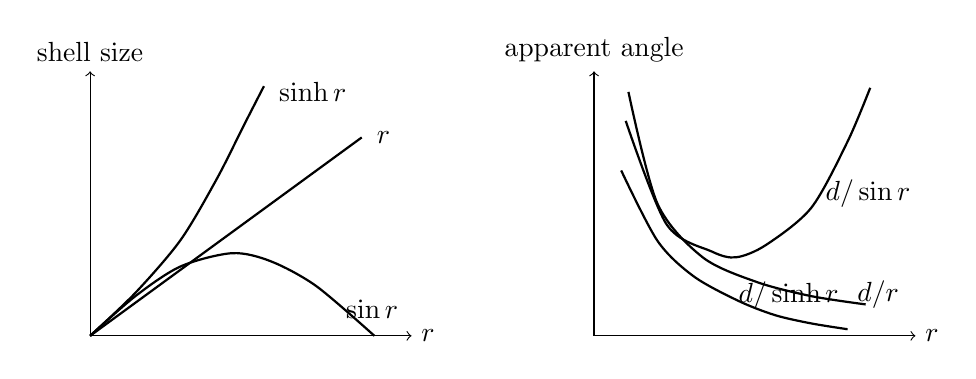
\begin{tikzpicture}[x=1.15cm,y=1.05cm]
\begin{scope}
\draw[->] (0,0)--(3.55,0) node[right] {$r$};
\draw[->] (0,0)--(0,3.2) node[above] {shell size};

\draw[thick] (0,0)--(3.0,2.4);
\draw (3.06,2.4) node[right] {$r$};

\draw[thick]
plot[smooth] coordinates {(0,0) (0.5,0.48) (1.0,0.84) (1.57,1.0) (2.0,0.9) (2.5,0.6) (3.14,0)};
\draw (2.72,0.55) node[below right] {$\sin r$};

\draw[thick]
plot[smooth] coordinates {(0,0) (0.5,0.52) (1.0,1.16) (1.4,1.9) (1.7,2.55) (1.92,3.02)};
\draw (1.98,2.95) node[right] {$\sinh r$};
\end{scope}

\begin{scope}[xshift=6.4cm]
\draw[->] (0,0)--(3.55,0) node[right] {$r$};
\draw[->] (0,0)--(0,3.2) node[above] {apparent angle};

\draw[thick]
plot[smooth] coordinates {(0.38,2.95) (0.7,1.6) (1.2,0.95) (1.8,0.65) (2.4,0.48) (3.0,0.38)};
\draw (2.8,0.5) node[right] {$d/r$};

\draw[thick]
plot[smooth] coordinates {(0.35,2.6) (0.8,1.35) (1.3,1.02) (1.57,0.95) (1.9,1.1) (2.4,1.55) (2.8,2.35) (3.05,3.0)};
\draw (2.45,1.72) node[right] {$d/\sin r$};

\draw[thick]
plot[smooth] coordinates {(0.3,2.0) (0.7,1.15) (1.1,0.72) (1.6,0.42) (2.0,0.25) (2.4,0.15) (2.8,0.08)};
\draw (2.15,0.2) node[above] {$d/\sinh r$};
\end{scope}
\end{tikzpicture}
}%
\caption{Los factores radiales de las capas y las correspondientes leyes del tamaño angular. La curvatura positiva hace que la capa se cierre; la negativa hace que crezca exponencialmente.}
\label{fig:c03-shell-angular-laws}
\end{figure}

\begin{classroomqa}\audiencequestion{¿Se vuelve infinito el valor de la coordenada radial al seguir recorriendo la esfera?}\lecturerresponse{No. En la esfera unitaria, \(r\) es la distancia angular geodésica y solo abarca el intervalo de \(0\) a \(\pi\). En \(r=\pi\), la capa ha colapsado en el punto antipodal. Aquí examinamos una geometría espacial fija; no seguimos un objeto que se desplaza hacia fuera en el tiempo. Más adelante, introducir un radio de curvatura multiplicará todas las distancias físicas por ese radio, pero no cambiará este intervalo adimensional. \lecturetimestamp{00:39:30--00:40:35}}\end{classroomqa}

\section{La proyección no es geometría}

Antes de pasar a la curvatura negativa, conviene ver cuánto puede deformarse una geometría fiel al representarla. Apoyemos una esfera sobre un plano tangente en el polo sur. Tracemos una recta desde el polo norte que pase por cada punto \(P\) de la esfera y prolonguémosla hasta el plano en \(P'\). Esta es la proyección estereográfica. El propio polo norte se proyecta al infinito. Una región pequeña cerca del polo sur se representa con poca distorsión, mientras que regiones intrínsecas iguales cerca del polo norte se vuelven enormes en el plano.

La distorsión pertenece al mapa, no a la esfera. La esfera original sigue siendo homogénea aunque su imagen plana asigne tamaños coordenados muy distintos a regiones equivalentes. Habrá que tener presente esta distinción cuando comprimamos un espacio hiperbólico infinito en un disco finito.

\begin{figure}[htbp]
\centering
\resizebox{\linewidth}{!}{%
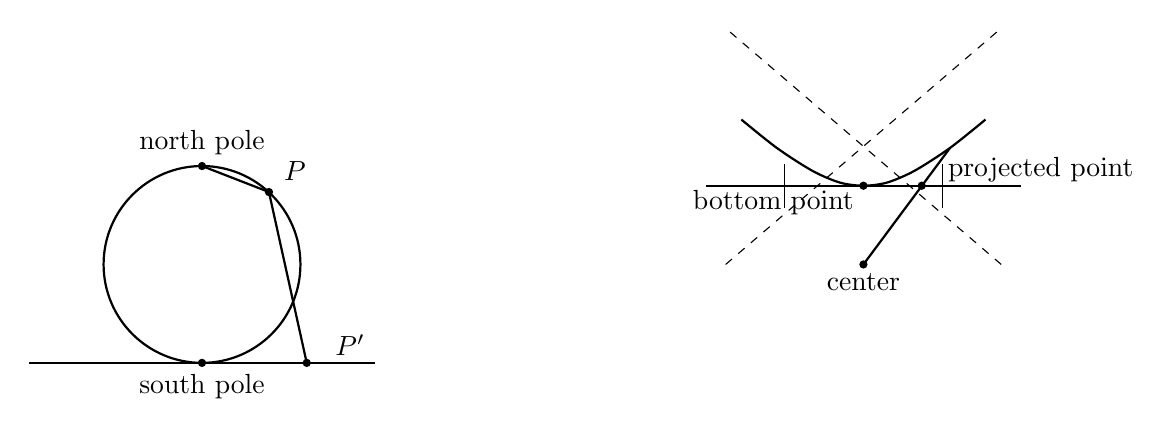
\begin{tikzpicture}[scale=1.0]
\begin{scope}[xshift=-4.2cm]
\draw[thick] (-2.2,-1.25)--(2.2,-1.25);
\draw[thick] (0,0) circle (1.25);
\fill (0,1.25) circle (1.5pt);
\fill (0,-1.25) circle (1.5pt);
\draw (0,1.55) node {north pole};
\draw (0,-1.55) node {south pole};

\fill (0.85,0.92) circle (1.5pt);
\draw (0.92,1.18) node[right] {$P$};
\draw[thick] (0,1.25)--(0.85,0.92)--(1.33,-1.25);
\fill (1.33,-1.25) circle (1.5pt);
\draw (1.57,-1.03) node[right] {$P'$};
\end{scope}

\begin{scope}[xshift=4.2cm]
\draw[thick] (-2.0,1)--(2.0,1);
\draw[dashed] (-1.75,0)--(1.75,3.0);
\draw[dashed] (1.75,0)--(-1.75,3.0);
\draw[thick]
plot[smooth] coordinates
{(-1.55,1.84) (-1.1,1.48) (-0.65,1.19) (-0.3,1.04) (0,1.0) (0.3,1.04) (0.65,1.19) (1.1,1.48) (1.55,1.84)};
\fill (0,0) circle (1.5pt);
\fill (0,1) circle (1.5pt);
\draw (0,-0.22) node {center};
\draw (0,0.78) node[left] {bottom point};
\draw[thick] (0,0)--(1.1,1.48);
\fill (0.74,1.0) circle (1.5pt);
\draw (0.95,1.2) node[right] {projected point};
\draw (-1,0.72) -- (-1,1.28);
\draw (1,0.72) -- (1,1.28);
\end{scope}
\end{tikzpicture}
}%
\caption{Izquierda: la proyección estereográfica envía el polo norte de una esfera al infinito. Derecha: un hiperboloide puede proyectarse en un disco finito, representado aquí mediante un intervalo transversal. La distorsión de las coordenadas no destruye la homogeneidad intrínseca.}
\label{fig:c03-projections}
\end{figure}

\section{Curvatura negativa: capas que crecen más que en el espacio plano}

La tercera geometría homogénea simplemente conexa sustituye \(\sin r\) por el seno hiperbólico. Sus métricas unitarias en dos y tres dimensiones son
\begin{equation}
dh_2^2 = dr^2 + \sinh^2 r\, d\Omega_1^2,
\label{eq:c03-hyperbolic-two}
\end{equation}
\begin{equation}
dh_3^2 = dr^2 + \sinh^2 r\, d\Omega_2^2.
\label{eq:c03-hyperbolic-three}
\end{equation}
La coordenada \(r\) abarca ahora
\begin{equation}
0\le r<\infty.
\end{equation}
Cerca del origen, \(\sinh r\approx r\), así que la geometría es localmente euclídea. Lejos del origen, sus capas crecen mucho más rápido que las capas euclídeas y nunca vuelven a contraerse.

La ley de crecimiento se deduce de
\begin{equation}
\sin r = \frac{e^{ir}-e^{-ir}}{2i},
\qquad
\sinh r = \frac{e^r-e^{-r}}{2}.
\label{eq:c03-sin-sinh}
\end{equation}
Para valores grandes de \(r\), se cumple \(\sinh r\sim e^r/2\). Por tanto, en dos dimensiones la circunferencia crece exponencialmente con el radio; en tres dimensiones, el área de la capa crece como \(\sinh^2r\sim e^{2r}/4\). Una distribución homogénea contiene, en consecuencia, muchos objetos en una capa lejana.

Para un objeto transversal de tamaño \(d\),
\begin{equation}
d^2 = \sinh^2 r\, d\theta^2,
\qquad\text{so}\qquad
d\theta = \frac{d}{\sinh r}.
\label{eq:c03-hyperbolic-angle}
\end{equation}
Cuando \(r\) es grande,
\begin{equation}
d\theta \sim 2d\,e^{-r}.
\end{equation}
Por tanto, la curvatura negativa produce una señal opuesta a la de la curvatura positiva: las reglas patrón lejanas parecen demasiado pequeñas, mientras que las capas lejanas contienen demasiados objetos en comparación con el espacio plano.

\begin{classroomqa}\audiencequestion{¿Cómo se distinguen el espacio esférico y el hiperbólico por sus intervalos radiales?}\lecturerresponse{En la esfera unitaria, \(r\) se detiene en el punto antipodal, \(r=\pi\). En el espacio hiperbólico, continúa sin límite: \(0\le r<\infty\). El factor de la capa muestra el mismo contraste: \(\sin r\) vuelve a cero, mientras que \(\sinh r\) crece indefinidamente. \lecturetimestamp{00:52:46--00:53:25}}\end{classroomqa}

Hay una incrustación que hace menos misteriosa la homogeneidad. Introduzcamos las coordenadas ambientales \(T,x,y\), donde \(T\) es solo una coordenada de incrustación y \emph{no} es el tiempo cosmológico, y tomemos la hoja superior
\begin{equation}
T^2 - x^2 - y^2 = 1.
\label{eq:c03-hyperboloid}
\end{equation}
Demos al espacio ambiente la métrica de signatura lorentziana
\begin{equation}
d\ell_{\mathrm{emb}}^2=-dT^2+dx^2+dy^2.
\label{eq:c03-ambient-minkowski}
\end{equation}
La métrica inducida en el hiperboloide es definida positiva. Las transformaciones de Lorentz conservan tanto la ecuación~\eqref{eq:c03-hyperboloid} como la~\eqref{eq:c03-ambient-minkowski}, y pueden llevar cualquier punto de la hoja superior a cualquier otro. En ese sentido, cambiar el origen en el espacio hiperbólico es como inclinar el eje temporal en el espacio ambiente auxiliar. Todos los puntos son geométricamente equivalentes.

Proyectemos el hiperboloide en un disco: los puntos infinitamente lejanos se acumulan en la circunferencia frontera. Las regiones cercanas se dibujan casi fielmente; las más lejanas se comprimen cada vez más. Esta es la representación del disco de Poincar\'e que aparece en las figuras repetitivas de ángeles y demonios. Una transformación de coordenadas puede llevar al centro una figura que parece diminuta cerca del borde, donde se vuelve grande, sin alterar las longitudes ni los ángulos intrínsecos. En tres dimensiones, el modelo correspondiente es una bola en vez de un disco. Los nombres \emph{Poincar\'eespacio}, \emph{espacio de Lobachevski} y \emph{espacio de curvatura negativa uniforme} se refieren a esta misma geometría local.

\begin{classroomqa}\audiencequestion{¿Se parece el disco finito a un diagrama de Penrose?}\lecturerresponse{Se parece en el sentido limitado de que un dominio infinito se representa dentro de una imagen finita. Sin embargo, aquí el disco representa solo el espacio, no el espacio-tiempo ni el infinito causal. Su frontera está infinitamente lejos según la métrica hiperbólica intrínseca, aunque el dibujo la sitúe a una distancia coordenada finita. \lecturetimestamp{01:02:55--01:03:05}}\end{classroomqa}

\section{El radio de curvatura}

Las métricas escritas hasta ahora describen geometrías unitarias. Para dar a una esfera o a un espacio hiperbólico un radio de curvatura arbitrario, se multiplica cada longitud por una constante. En la pizarra, esa constante se denota \(a\); para evitar confundirla con el factor de escala cosmológico dependiente del tiempo que usaremos más adelante, llamaremos \(R_c\) al radio de curvatura estático. Como la métrica mide longitudes al cuadrado,
\begin{align}
ds_{\mathrm{sph}}^2
  &=R_c^2d\Omega_n^2
   =R_c^2\left(dr^2+\sin^2r\,d\Omega_{n-1}^2\right),\\
ds_{\mathrm{hyp}}^2
  &=R_c^2dh_n^2
   =R_c^2\left(dr^2+\sinh^2r\,d\Omega_{n-1}^2\right).
\label{eq:c03-scaled-curvature}
\end{align}
La distancia radial física es \(R_cr\). Al aumentar \(R_c\), el espacio se curva menos; la magnitud de la curvatura seccional constante varía como \(1/R_c^2\). En el límite \(R_c\to\infty\), ambas métricas curvas se aproximan a la geometría euclídea en toda región finita fija.

\begin{classroomqa}\audiencequestion{Si se duplica el tamaño de la esfera, ¿se curva más o menos?}\lecturerresponse{Menos. La primera respuesta que se dio en clase se corrigió al comparar una pelota de baloncesto con la Tierra: la superficie más pequeña se curva más rápidamente a lo largo de una distancia dada. Al duplicar \(R_c\), la escala de curvatura inversamente proporcional al radio se reduce a la mitad y la curvatura seccional \(1/R_c^2\) se divide por cuatro. \lecturetimestamp{01:10:14--01:10:56}}\end{classroomqa}

Esto explica por qué las tres geometrías se parecen en las proximidades. Para \(r\ll1\),
\begin{equation}
\sin r=r-\frac{r^3}{6}+\cdots,
\qquad
\sinh r=r+\frac{r^3}{6}+\cdots.
\end{equation}
El término principal de ambas métricas curvas es la métrica polar plana; la curvatura aparece por primera vez en correcciones relativas de orden \((L/R_c)^2\) a lo largo de una escala física \(L\).

\begin{classroomqa}\audiencequestion{¿Las observaciones nos dicen si el espacio es plano, esférico o hiperbólico?}\lecturerresponse{Nos dicen que la región observable es muy cercana a plana. La estimación aproximada dada en clase fue que un límite del uno por ciento en los efectos de la curvatura implica que \(R_c\) mide al menos unas diez veces el tamaño de la región visible, porque \((L/R_c)^2\lesssim10^{-2}\). El volumen de curvatura correspondiente sería entonces de al menos aproximadamente \(10^3\) volúmenes visibles. Esta es una estimación de orden de magnitud expuesta en clase, no una cita de datos de precisión actuales, y la planitud exacta sigue siendo la posibilidad \(R_c=\infty\). \lecturetimestamp{01:11:00--01:13:37}}\end{classroomqa}

\section{Plano pero finito: el toro}

Ahora debemos corregir la afirmación de que los espacios plano, esférico e hiperbólico son las únicas posibilidades homogéneas. Son las tres geometrías simplemente conexas de curvatura constante. Un espacio plano también puede tener una topología global no trivial.

Empecemos con un rectángulo euclídeo. Identifiquemos punto por punto su lado izquierdo con el derecho, y su borde inferior con el superior. Al cruzar cualquier borde, se reaparece por el opuesto. La métrica local sigue siendo \(dx^2+dy^2\), pero el espacio global es periódico y finito. Este cociente es un toro plano bidimensional \(T^2\). Una dimensión periódica da un círculo \(T^1\); al identificar las caras opuestas de una caja rectangular se obtiene un toro plano tridimensional \(T^3\), y la construcción se extiende a cualquier número de dimensiones.

\begin{figure}[htbp]
\centering
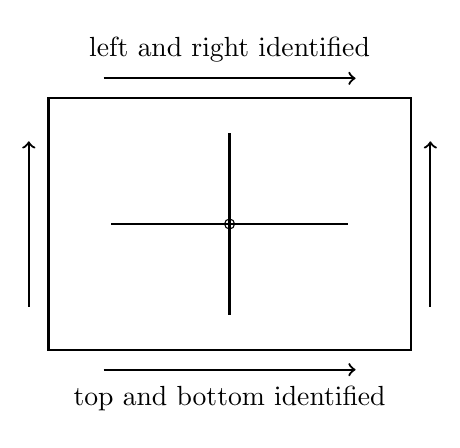
\begin{tikzpicture}[scale=1.0]
\draw[thick] (0,0) rectangle (4.6,3.2);

\draw[->,thick] (0.7,3.45)--(3.9,3.45);
\draw[->,thick] (0.7,-0.25)--(3.9,-0.25);

\draw[->,thick] (-0.25,0.55)--(-0.25,2.65);
\draw[->,thick] (4.85,0.55)--(4.85,2.65);

\draw[thick] (0.8,1.6)--(3.8,1.6);
\draw[thick] (2.3,0.45)--(2.3,2.75);

\draw (2.3,1.6) circle (1.8pt);

\draw (2.3,-0.62) node {top and bottom identified};
\draw (2.3,3.82) node {left and right identified};
\end{tikzpicture}
\caption{Un toro plano construido al identificar los lados opuestos de un rectángulo. Los lados no son fronteras: los puntos emparejados son el mismo punto del espacio cociente.}
\label{fig:c03-flat-torus}
\end{figure}

\begin{classroomqa}\audiencequestion{¿Puede, entonces, un universo ser plano y finito a la vez?}\lecturerresponse{Sí. La planitud es una afirmación local sobre la métrica; la finitud puede ser una afirmación global sobre la topología. Un toro tridimensional lo bastante grande parecería euclídeo en toda la región que podemos observar, aunque su volumen total fuera finito. \lecturetimestamp{01:13:37--01:17:59}}\end{classroomqa}

La representación mediante el recubrimiento universal deja clara la consecuencia observable. En vez de identificar los bordes, teselamos un plano euclídeo infinito con copias del rectángulo fundamental. Un mismo objeto del toro aparece una vez en cada copia. En tres dimensiones, las copias forman una disposición periódica parecida a un cristal.

\begin{classroomqa}\audiencequestion{¿Podríamos vivir en un universo toroidal sin darnos cuenta?}\lecturerresponse{Sí, si la celda fundamental es mayor que la región desde la que nos ha llegado luz. Si fuera lo bastante pequeña, la luz podría atravesar las identificaciones y veríamos imágenes repetidas de las mismas galaxias, quizá incluso vistas repetidas de nuestro propio entorno, en distintas direcciones. En ambos casos, la geometría local seguiría siendo plana. \lecturetimestamp{01:18:16--01:22:04}}\end{classroomqa}

\begin{classroomqa}\audiencequestion{¿Por qué la esfera termina en su punto antipodal mientras que el toro se repite?}\lecturerresponse{En la esfera, la capa circundante realmente se encoge hasta tamaño cero en \(r=\pi\); todas las direcciones radiales se encuentran en el punto antipodal. En un toro, el borde de una celda rectangular elegida nunca se encoge. Se identifica con un borde opuesto de igual tamaño, de modo que cruzarlo prolonga el mismo espacio en una descripción mediante coordenadas periódicas. \lecturetimestamp{01:22:06--01:23:02}}\end{classroomqa}

\section{Del espacio al espacio-tiempo}

Ahora podemos volver a introducir el tiempo. En unidades en las que la velocidad de la luz \(c=1\), la métrica de Minkowski es
\begin{equation}
ds^2 = -dt^2 + dx^2 + dy^2 + dz^2.
\label{eq:c03-minkowski}
\end{equation}
La elección de la convención de signos es arbitraria; lo que importa es que el término temporal tenga signo opuesto al de los términos espaciales. Un rayo de luz sigue una trayectoria nula:
\begin{equation}
ds^2 = 0.
\end{equation}
Para el movimiento únicamente a lo largo de \(x\),
\begin{equation}
-dt^2 + dx^2 = 0
\qquad\Rightarrow\qquad
dx = \pm dt.
\label{eq:c03-null-flat}
\end{equation}
Los dos signos describen la luz que se mueve hacia la izquierda o hacia la derecha con rapidez unitaria.

En cosmología, conservemos el término de tiempo propio \(-dt^2\), sustituyamos la parte espacial euclídea por una métrica espacial homogénea y dejemos que su escala global varíe con el tiempo. Denotamos este factor de escala por \(a(t)\). Ahora es una función dinámica, no el radio fijo \(R_c\) que usamos en la comparación estática.

Como ejemplo de \(2+1\) dimensiones que se puede visualizar, tomemos
\begin{equation}
ds^2 = -dt^2 + a(t)^2 d\Omega_2^2.
\label{eq:c03-two-plus-one}
\end{equation}
En cada instante fijo \(t\), el espacio es una esfera \(2\) de radio \(a(t)\). Al apilar estas esferas en el tiempo se obtiene el espacio-tiempo. La construcción familiar en \(3+1\) dimensiones es
\begin{equation}
ds^2 = -dt^2 + a(t)^2 d\Sigma^2,
\label{eq:c03-frw-general}
\end{equation}
donde \(d\Sigma^2\) es una métrica espacial unitaria e independiente del tiempo. Los tres casos simplemente conexos son
\begin{align}
\text{flat:}\quad
ds^2&=-dt^2+a(t)^2\left(dx^2+dy^2+dz^2\right),\label{eq:c03-frw-flat}\\
\text{spherical:}\quad
ds^2&=-dt^2+a(t)^2d\Omega_3^2,\label{eq:c03-frw-spherical}\\
\text{hyperbolic:}\quad
ds^2&=-dt^2+a(t)^2dh_3^2.\label{eq:c03-frw-hyperbolic}
\end{align}
La escala relativa de las coordenadas comóviles permanece fija mientras cambia \(a(t)\). En las normalizaciones esférica e hiperbólica, \(a(t)\) también es el radio de curvatura instantáneo. En el caso plano, la normalización absoluta puede absorberse en las coordenadas comóviles.

La ley de Hubble se obtiene antes de imponer cualquier ecuación de campo gravitatorio. Consideremos dos puntos comóviles próximos con una separación coordenada fija \(\chi\). Su separación física es
\begin{equation}
D(t)=a(t)\chi.
\label{eq:c03-comoving-distance}
\end{equation}
Al derivar manteniendo fijo \(\chi\), se obtiene
\begin{equation}
V=\dot D=\dot a(t)\chi.
\end{equation}
Eliminando \(\chi\),
\begin{equation}
V = \frac{\dot a}{a} D.
\label{eq:c03-hubble-law}
\end{equation}
Así,
\begin{equation}
H = \frac{\dot a}{a}.
\label{eq:c03-hubble-parameter}
\end{equation}
Esta es una identidad cinemática válida para la expansión o contracción homogénea. Se cumple para las tres geometrías espaciales: \(\dot a>0\) implica recesión y \(\dot a<0\) implica acercamiento.

La geometría por sí sola no determina \(a(t)\). Funciones como
\begin{equation}
a(t)\propto t^{2/3},
\qquad
a(t)\propto t^{1/2},
\qquad
a(t)\propto e^{Ht}
\end{equation}
cumplen todas la forma métrica homogénea, pero describen contenidos cósmicos de materia y energía diferentes. La relatividad general proporciona la ecuación dinámica que permite seleccionar entre ellas. La ecuación de Friedmann resultante también relacionará los casos plano, esférico e hiperbólico con las alternativas de energía nula, negativa y positiva de la cosmología newtoniana desarrollada anteriormente.

\begin{classroomqa}
\audiencequestion{¿Podrían la geometría y la evolución cósmica ser mucho más complicadas que las de estos modelos?}
\lecturerresponse{Desde luego. La homogeneidad y la isotropía son hipótesis restrictivas, elegidas porque resultan naturales, concuerdan con las observaciones a gran escala y son manejables matemáticamente. Existen muchas geometrías y evoluciones más complicadas. Una cuestión dinámica importante es si amplias clases de modelos inicialmente irregulares evolucionan hacia una de estas formas homogéneas simples. \lecturetimestamp{01:36:00--01:36:50}}
\end{classroomqa}

\begin{classroomqa}
\audiencequestion{¿Es la \(3\)-esfera el borde de un objeto de cuatro dimensiones?}
\lecturerresponse{Puede representarse así mediante una inmersión, pero el espacio cosmológico es la \(3\)-esfera misma. Tiene tres dimensiones intrínsecas y no tiene borde. La representación euclídea de cuatro dimensiones es un recurso auxiliar opcional; la ecuación~\eqref{eq:c03-three-sphere} ya define la geometría por completo. \lecturetimestamp{01:36:55--01:37:59}}
\end{classroomqa}

\begin{classroomqa}
\audiencequestion{¿Es la luminosidad la única forma de obtener la distancia necesaria para comprobar la curvatura?}
\lecturerresponse{No. Las líneas espectrales permiten identificar el corrimiento al rojo, las escalas de distancias locales calibran la relación de Hubble y las supernovas proporcionan luminosidades aproximadamente estándar. Estos métodos se contrastan entre sí, en lugar de confiar en cada uno por separado. Incluso la ley de luminosidad del inverso del cuadrado depende de la geometría, porque el área del frente de luz viene determinada por \(r^2\), \(\sin^2r\) o \(\sinh^2r\). Es la concordancia entre varias magnitudes observables lo que respalda que el universo sea casi plano. \lecturetimestamp{01:38:00--01:41:07}}
\end{classroomqa}

\section{Qué conviene recordar}

La geometría de un universo homogéneo puede deducirse del crecimiento de las capas esféricas alrededor de cualquier observador:
\begin{equation}
f(r)=
\begin{cases}
r, & \text{flat space},\\
\sin r, & \text{positive curvature},\\
\sinh r, & \text{negative curvature}.
\end{cases}
\end{equation}
La métrica espacial es \(dr^2+f(r)^2d\Omega_{n-1}^2\). La misma función determina los tamaños angulares y la cantidad de objetos disponibles en una capa, por lo que la curvatura tiene un significado observacional directo. Un radio de curvatura grande oculta localmente estas diferencias, y una identificación toroidal muestra que la curvatura local no determina por sí sola el tamaño global ni la topología.

Al añadir \(-dt^2\) y el factor común \(a(t)^2\) a cualquiera de las tres métricas espaciales homogéneas, se obtiene un espacio-tiempo cosmológico. De inmediato se deduce \(V=HD\), con \(H=\dot a/a\), pero \(a(t)\) queda indeterminado. Por tanto, el siguiente paso no consiste en otro ejercicio de geometría. Se trata del problema dinámico: usar las ecuaciones de Einstein para determinar cómo la materia, la radiación, la curvatura y otras formas de energía hacen evolucionar el factor de escala.
